\documentclass[a4paper,11pt]{article}
%\usepackage[T1]{fontenc}

%\setlength{\textwidth}{20cm}
%\setlength{\marginparwidth}{0cm}
%\setlength{\voffset}{0cm}
\usepackage[utf8]{inputenc}
\usepackage[francais]{babel}
\usepackage{amsmath}
\usepackage{graphicx}
\usepackage{listings}
\usepackage{xcolor}
\usepackage{caption}
\usepackage{subcaption}
\usepackage{subfig}


%==== to fix locations of figures and tables
\usepackage{float}
\usepackage{placeins}

\lstset{
language=VHDL,
basicstyle=\small\sffamily,
numbers=left,
numberstyle=\tiny,
frame=tb,
columns=fullflexible,
showstringspaces=false
}
%\special{papersize=210mm,297mm}

\title{{\Huge Electronique numérique}\\Initiation à VHDL (1/3)\\CORRECTIONS}
%\title{TD1}
\date{}

\begin{document}
\maketitle
\begin{enumerate}
  \item Dessiner l'enveloppe externe du composant décrit par cette entité.
  \textcolor{red}{Voir figure \ref{moncircuit}}.
  \begin{figure}
    \centering
    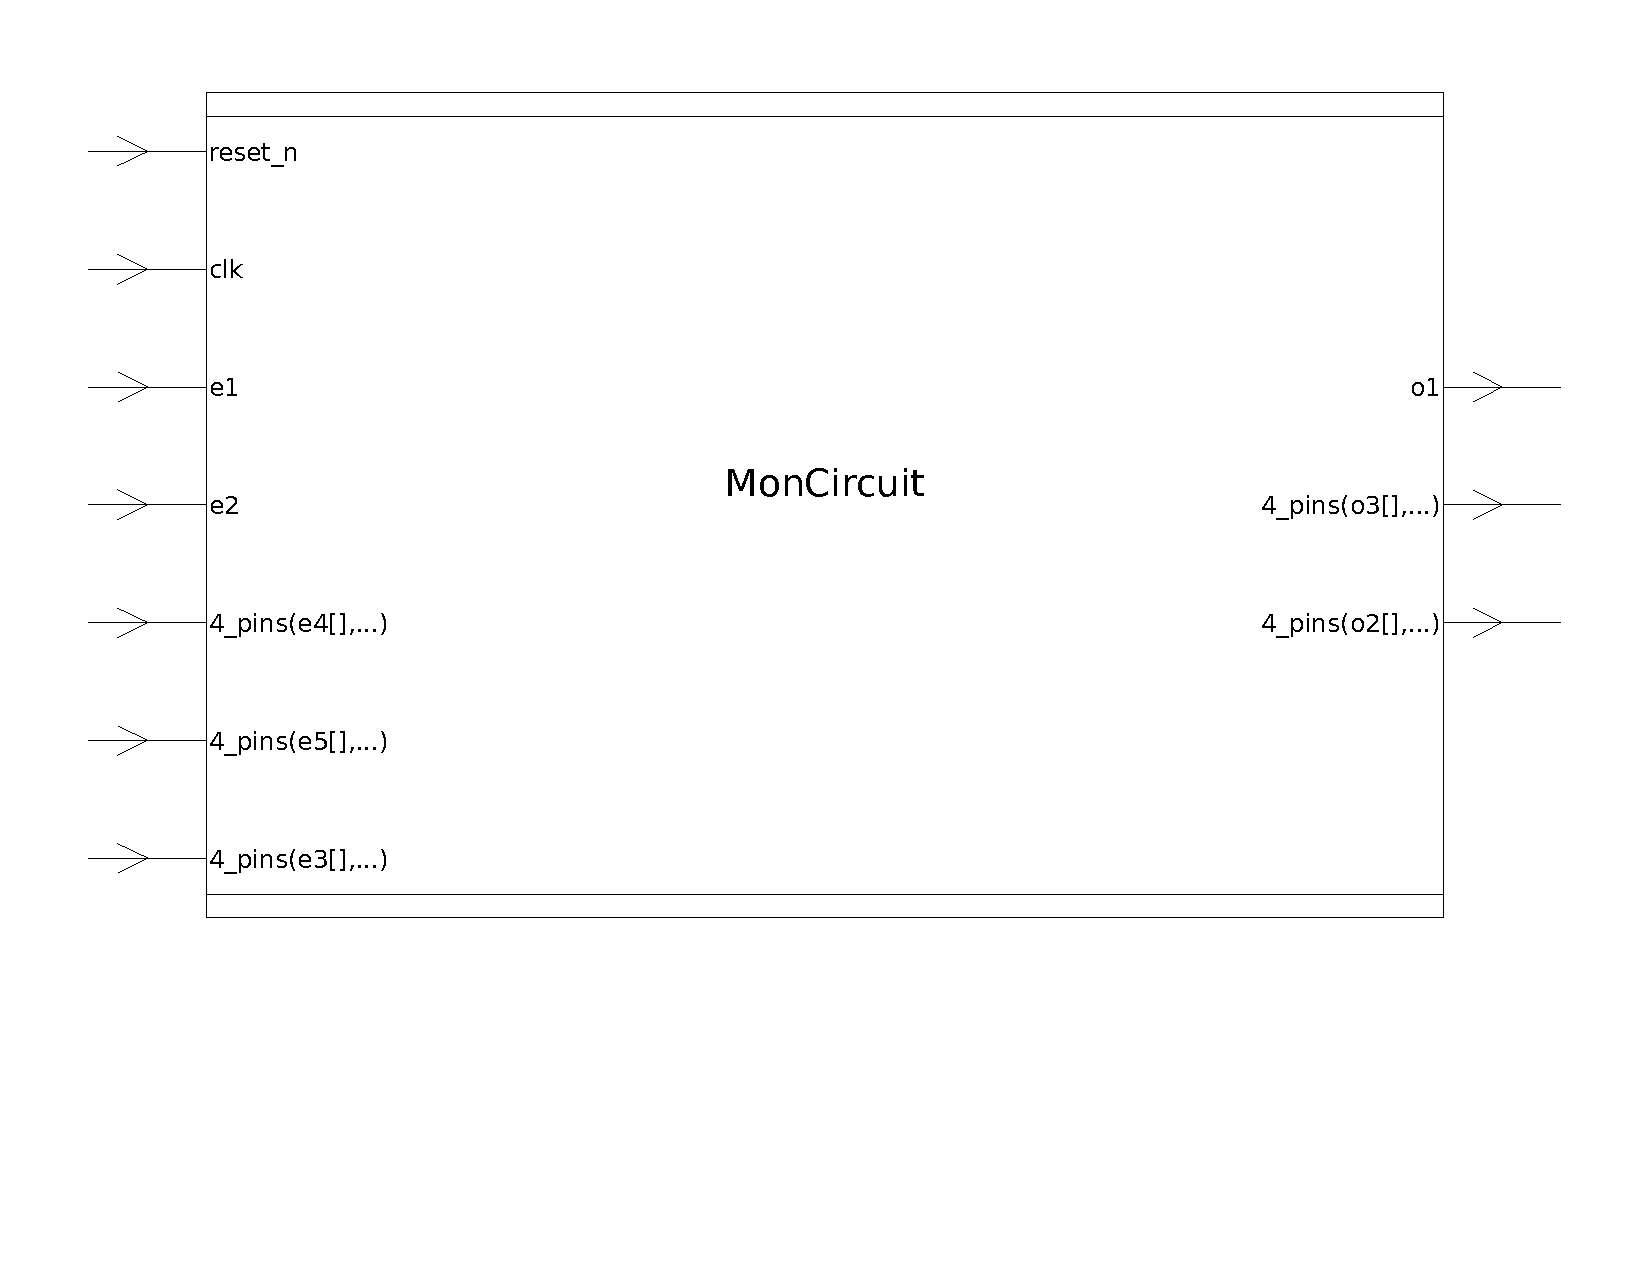
\includegraphics[width=5cm]{./code/entity_mon_circuit.pdf}
    \caption{Entity du composant MonCircuit}
    \label{moncircuit}
  \end{figure}

  \item Dessiner l'entité d'un demi-additionneur, puis le code VHDL de cette entité.
  \textcolor{red}{Voir figure \ref{fig:ha}}
  \item Rappeler la constitution interne du demi-additionneur.
  \textcolor{red}{Voir figure \ref{fig:ha}}

  \begin{figure}
    \centering
    \begin{subfigure}{.5\textwidth}
      \centering
      %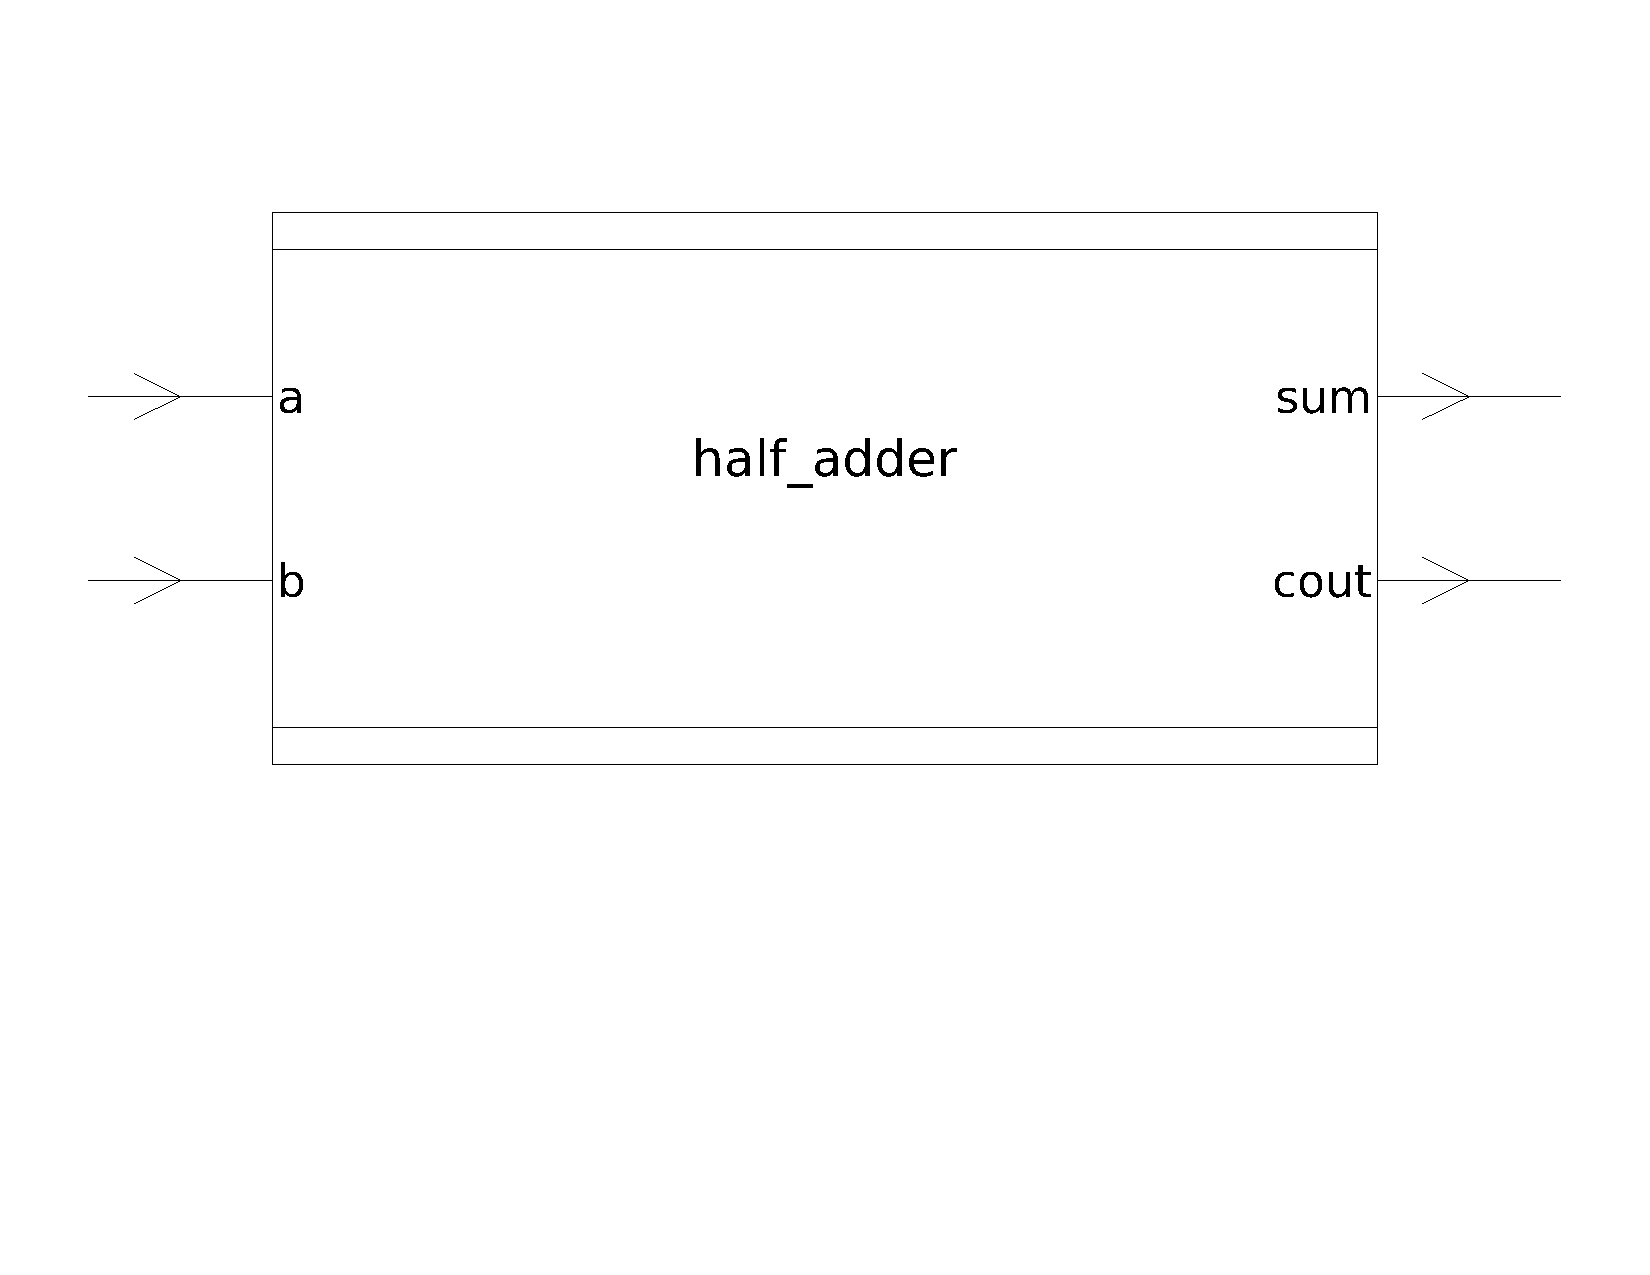
\includegraphics[width=.4\linewidth]{./code/entity_half_adder.pdf}
      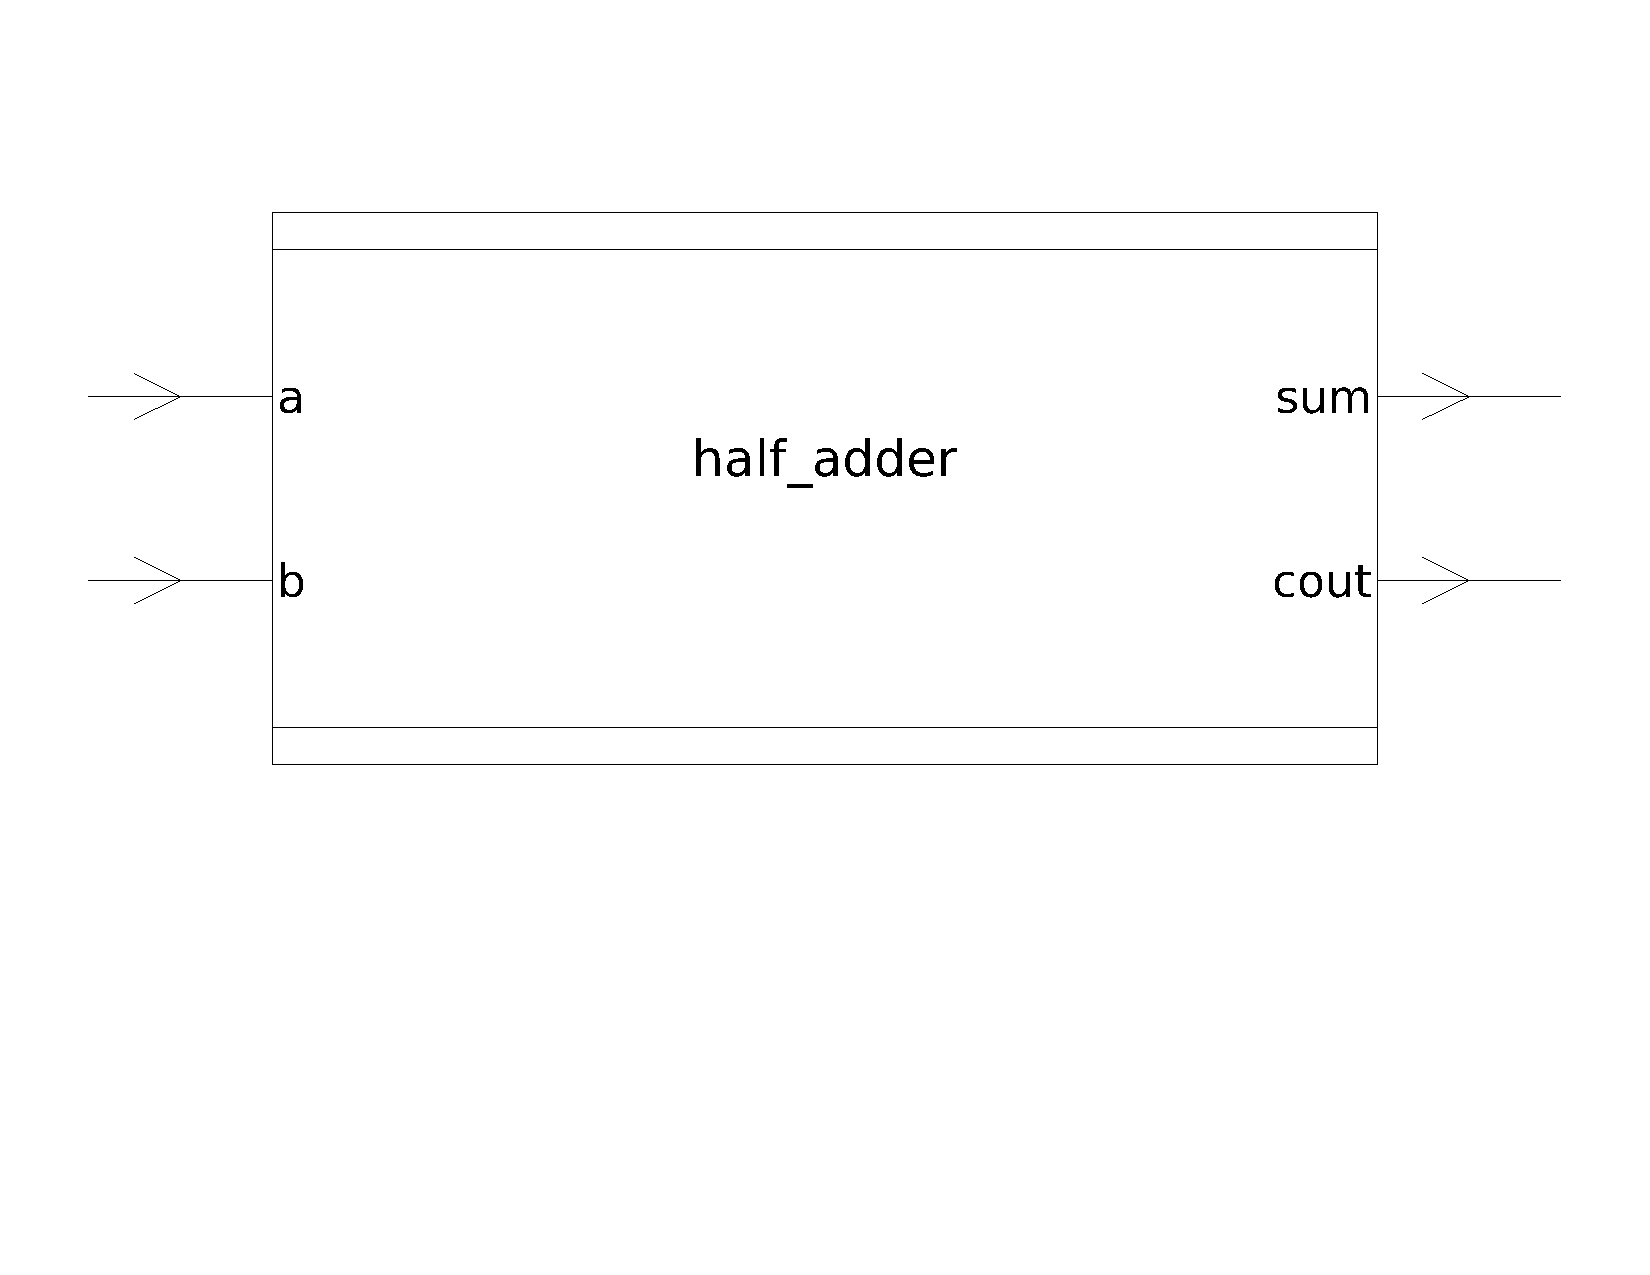
\includegraphics[width=6cm]{./code/entity_half_adder.pdf}
      %\caption{A subfigure}
      %\label{fig:sub1}
    \end{subfigure}%
    \begin{subfigure}{.5\textwidth}
      \centering
      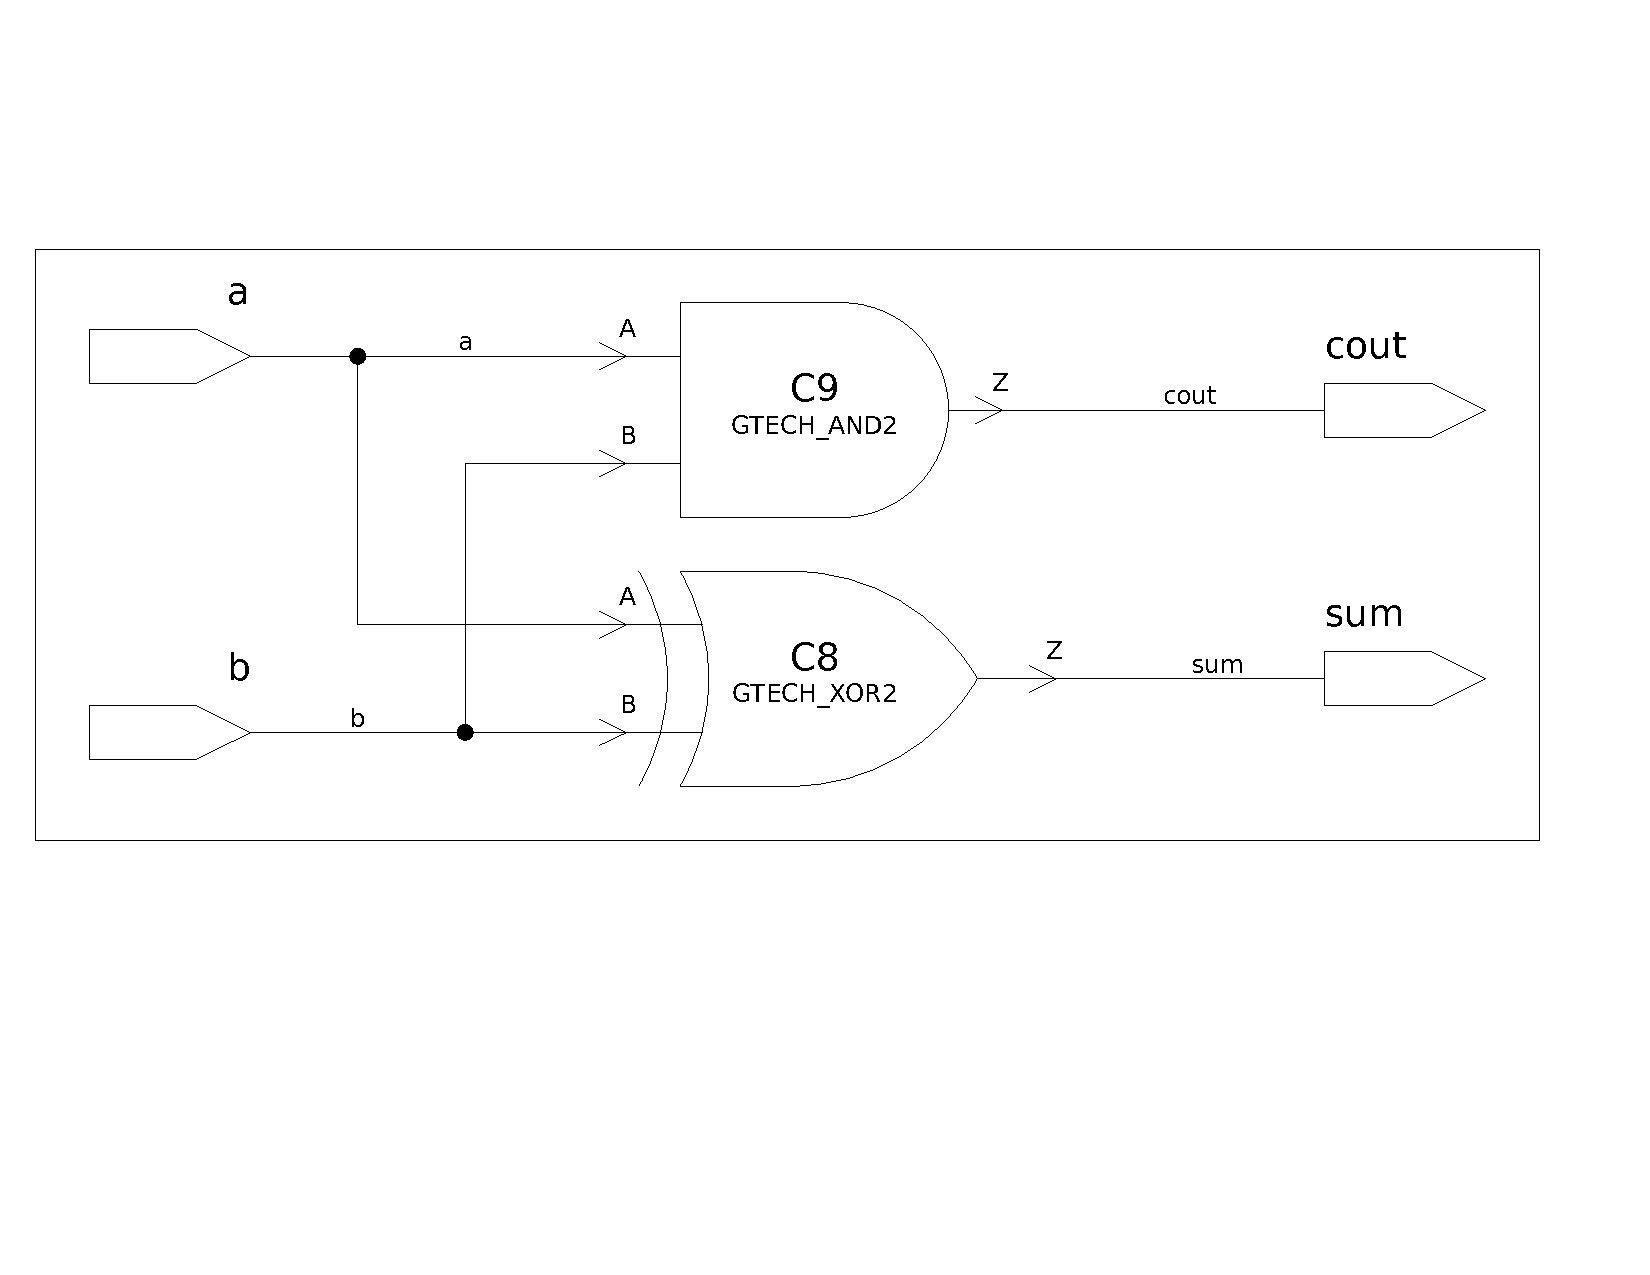
\includegraphics[width=7cm]{./code/arch_half_adder.pdf}
      % \caption{A subfigure}
      % \label{fig:sub2}
    \end{subfigure}
    \caption{Entité et architecture du demi-additionneur 1 bit}
    \label{fig:ha}
  \end{figure}

  \item Coder l'architecture de ce demi-additionneur.
    \lstset{inputencoding=utf8}
    \lstinputlisting[language=VHDL]{./code/half_adder.vhd}

  \item Dessinez la constitution interne d'un additionneur 1 bit complet, à partir du demi-additionneur.
  \begin{figure}
    \centering
    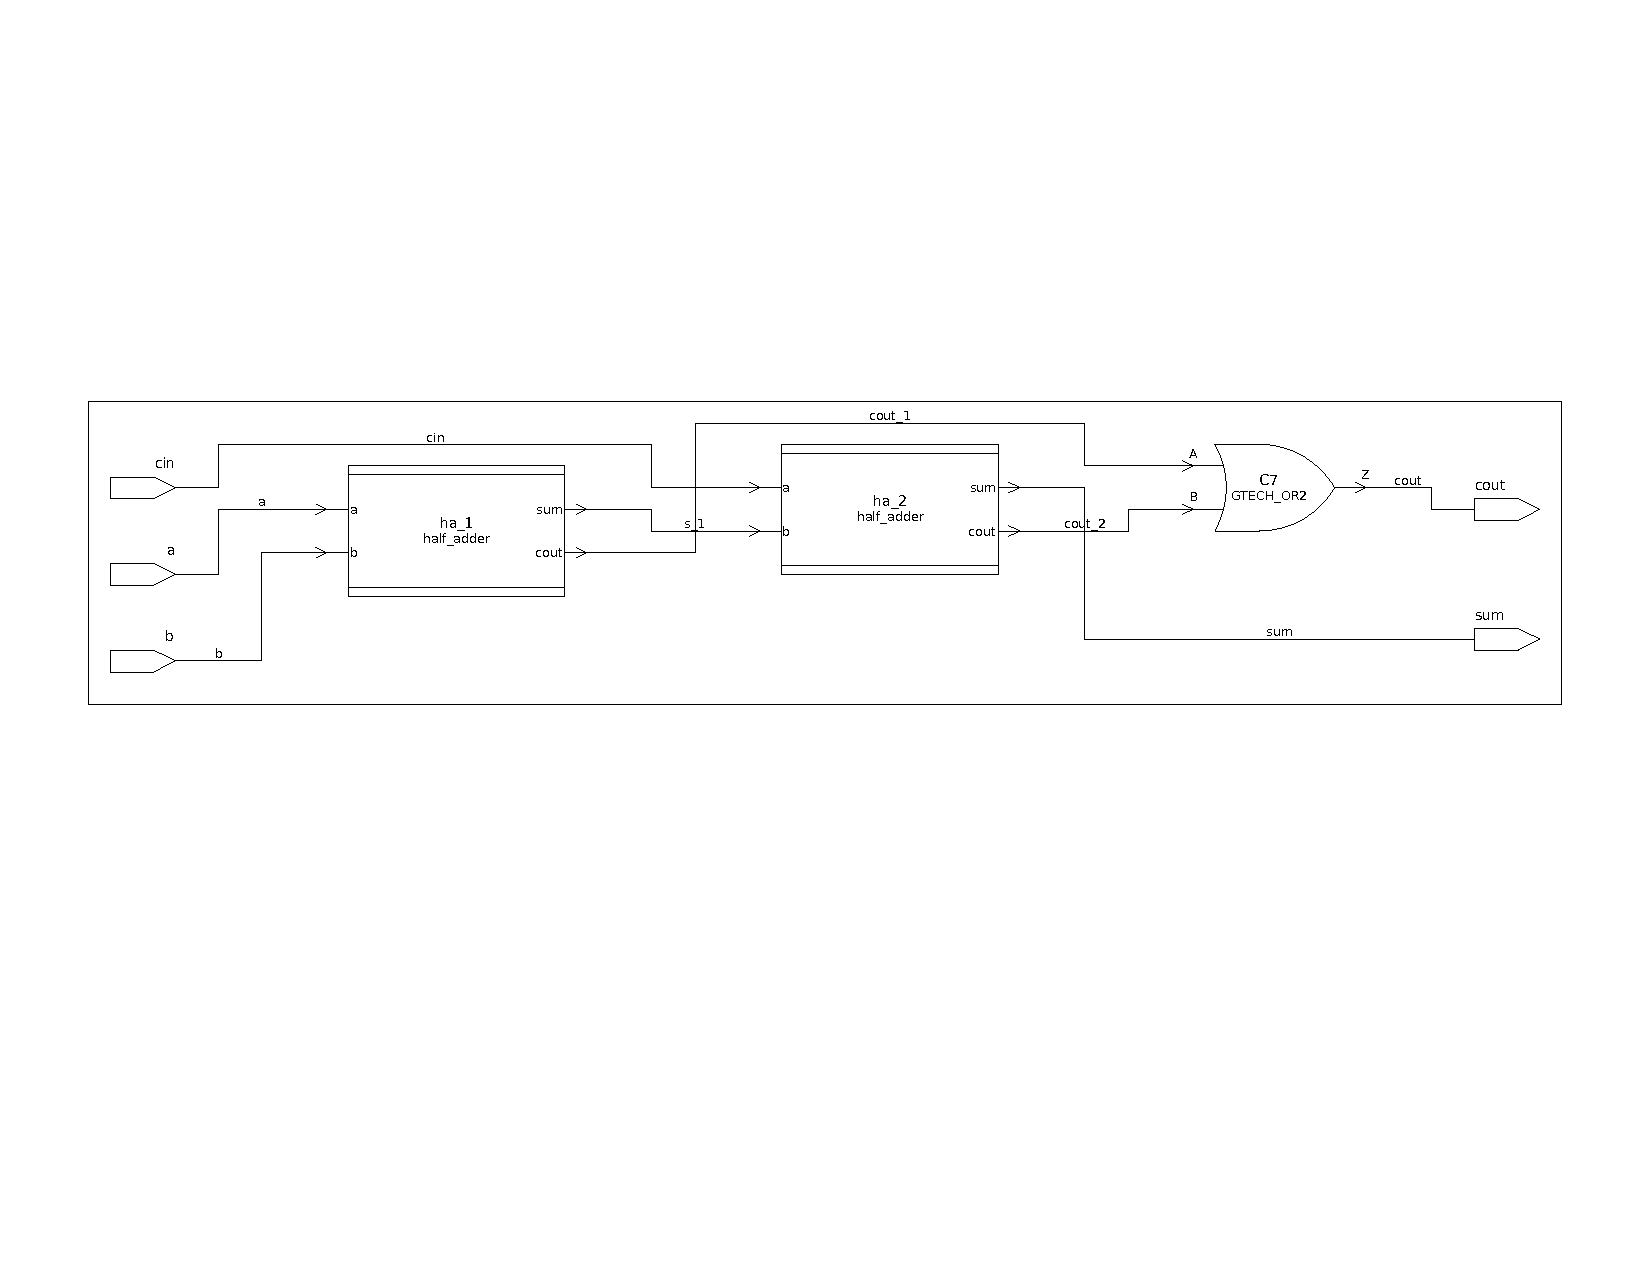
\includegraphics[width=10cm]{./code/arch_full_adder.pdf}
    \caption{Architecture du demi-additionneur 1 bit}
    \label{fig:ha}
  \end{figure}

  \item Coder en VHDL l'architecture de cet additionneur 1 bit.
  \lstinputlisting[language=VHDL]{./code/full_adder.vhd}

  \item Coder en VHDL l'entité et l'architecture d'un additionneur 8 bits.
  \lstinputlisting[language=VHDL]{./code/adder8b.vhd}
  \begin{figure}
    \centering
    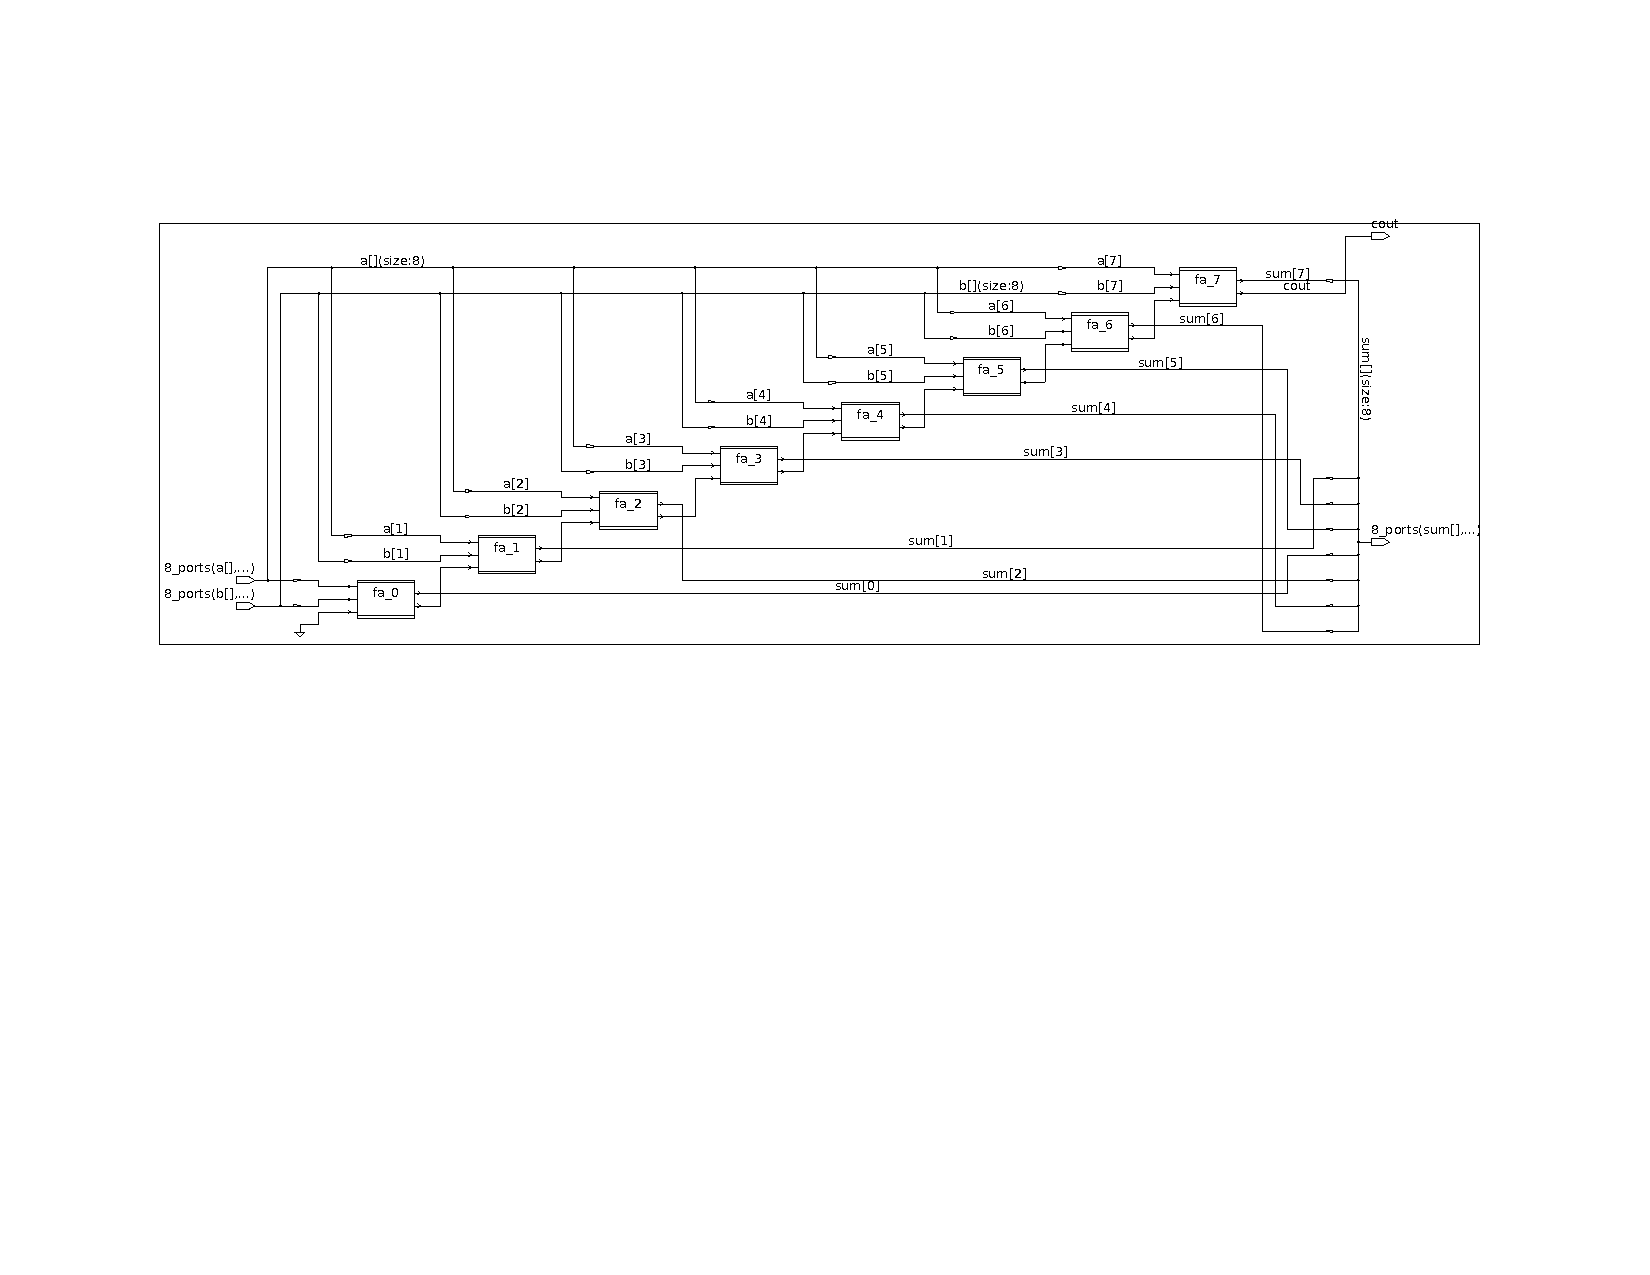
\includegraphics[width=15cm]{./code/arch_adder8b.pdf}
    \caption{Architecture de l'additionneur 8 bits}
    \label{fig:ha}
  \end{figure}

  \item Le testbench présente également une entité. Localisez cette entité. En quoi est-elle particulière ? Comment peut-on l'expliquer ?

      \textcolor{red}{Un tel banc de test possède une entité {\it vide} :
      elle ne possède aucune entrée, ni sortie. C'est le laboratoire, portes closes.}

  \item Un générateur d'horloge est contenu dans le banc de test. Combien de lignes sont nécessaires ? Dessinez le chronogramme de cette horloge.

    \textcolor{red}{Une seule ligne suffit. On inverse le signal tous les demi-période d'horloge, à l'aide d'une assignation conditionnée par un signal
"running", qui nous permettra de contrôler l'arrêt de la simulation}

  \item Comment notre banc de test provoque t-il concrètement cet arrêt ?
\textcolor{red}{Le signal running est affecté à "false" à la fin du processus de stimulation. Plus aucun événement n'est crée par le simulateur.}

  \item Dessiner le chronogramme des stimuli.
  \begin{figure}
    \centering
    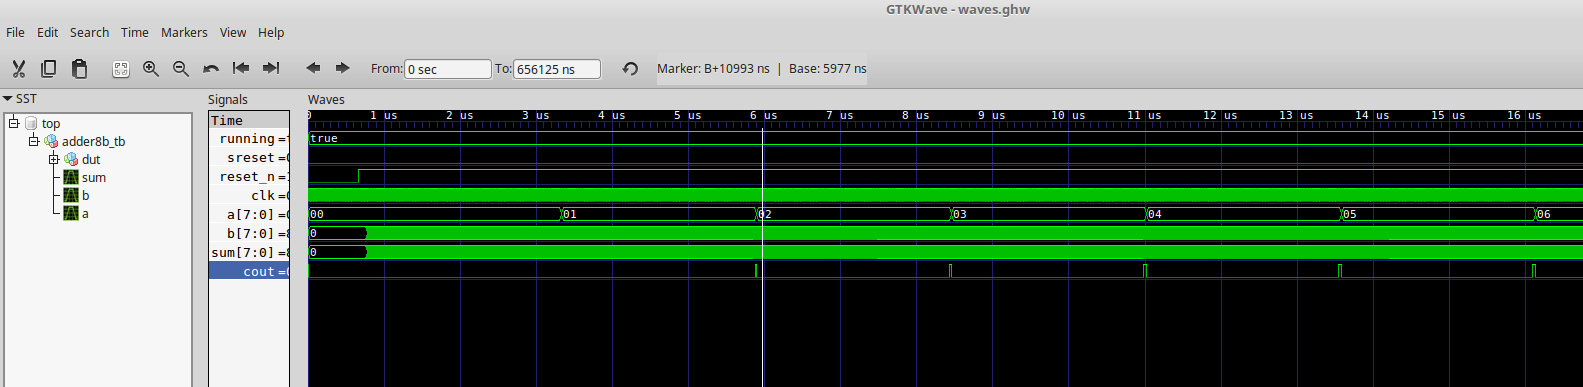
\includegraphics[width=15cm]{./code/gtkwave_adder8b.png}
    \caption{Chronogramme (overview)}
    \label{fig:signed}
  \end{figure}

  \begin{figure}
    \centering
    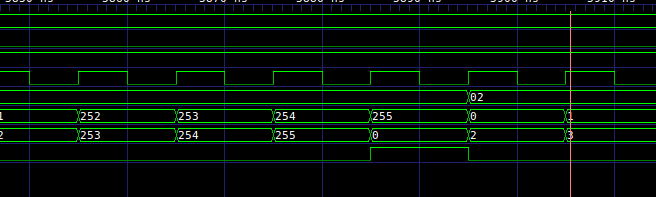
\includegraphics[width=15cm]{./code/gtkwave_adder8b_1_255.png}
    \caption{Chronogramme : cas de $1+255$}
    \label{fig:signed}
  \end{figure}

  \item L'additionneur fonctionne-t-il avec des nombres signés ?
\textcolor{red}{Oui ! En tous les cas, un test semble aller en ce sens ! Voir figure \ref{signed}.}
\begin{figure}
  \centering
  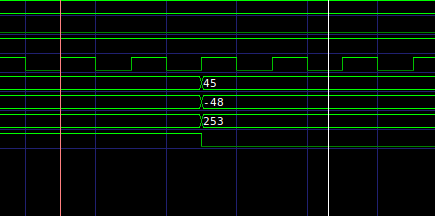
\includegraphics[width=15cm]{./code/signed_values.png}
  \caption{L'additionneur fonctionne pour les nombres signés.}
  \label{fig:signed}
\end{figure}
\end{enumerate}


\section{Script de compilation}

Script de compilation GHDL (donné sous Moodle):
\begin{verbatim}
  echo "=> cleaning..."
  rm -rf waves.ghw *.o
  echo "=> analyzing VHDL files..."
  ghdl -a half_adder.vhd
  ghdl -a full_adder.vhd
  ghdl -a adder8b.vhd
  ghdl -a adder8b_tb.vhd
  echo "=> elaboration..."
  ghdl -e adder8b_tb
  echo "=> running simulation"
  ghdl -r adder8b_tb --wave=waves.ghw
  echo "=> starting waveform viewer"
  gtkwave waves.ghw chrono.sav
\end{verbatim}

Testbench (donné sous Moodle) :

\lstset{inputencoding=utf8}
\lstinputlisting[language=VHDL]{./code/adder8b_tb.vhd}

\section{Using generate}
\lstset{inputencoding=utf8}
\lstinputlisting[language=VHDL]{./code/adder8b_generate.vhd}


\end{document}
